\documentclass[10pt,landscape,a4paper]{article}
\usepackage[utf8]{inputenc}
\usepackage[english]{babel}
\usepackage[utopia,sfscaled]{mathdesign}
\usepackage{multicol}
\usepackage[top=2mm,bottom=2mm,left=3mm,right=3mm]{geometry}
\usepackage{lipsum}
\usepackage{microtype}
\usepackage{graphicx}
\usepackage{amsmath}
\usepackage{breqn}
\usepackage{enumitem}
\usepackage{titlesec}
\usepackage{minted}

\setitemize{noitemsep,topsep=0pt,parsep=0pt,partopsep=0pt}
\setenumerate{noitemsep,topsep=0pt,parsep=0pt,partopsep=0pt}
\setlength{\parindent}{0pt}
\setlength{\parskip}{0.2\baselineskip}
\titleformat*{\section}{\footnotesize\bfseries}
\titleformat*{\subsection}{\scriptsize\bfseries}
\titlespacing{\section}{0pt}{\parskip}{-\parskip}
\titlespacing{\subsection}{0pt}{\parskip}{-\parskip}

\graphicspath{{image/}}

% TODO: Add BTree, BSTree, and BSTree2
% TODO: Add tutorial solutions
% TODO: Add variants of dutch flag

\begin{document}
\tiny

\newmintedfile[prologFile]{prolog}{linenos=true,firstnumber=1,numbersep=2pt,breaklines=true}
\newmintedfile[haskellFile]{haskell}{linenos=true,firstnumber=1,numbersep=2pt,breaklines=true}

\begin{multicols*}{5}

\section{Prolog}

\subsection*{Sample Box Model}
\prologFile[firstline=6,lastline=19]{code/sillyeg.pl}
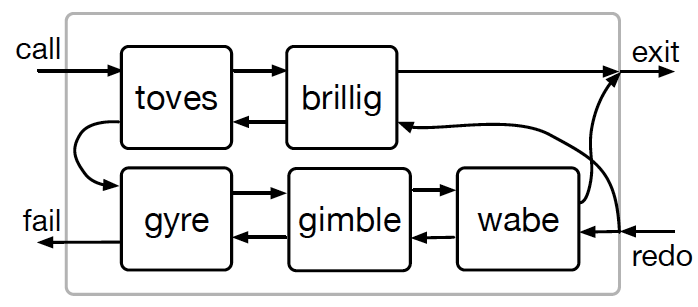
\includegraphics[scale=0.15]{box_model}

\subsection*{Delete Exactly 1 Elements}
\prologFile[firstline=41,lastline=45]{code/as3sol.pl}

\subsection*{Replace}
\prologFile[firstline=55,lastline=61]{code/mid1asol.pl}

\subsection*{Flatten}
\prologFile[firstline=71,lastline=73]{code/mid2sol.pl}

\subsection*{Derivative}
\prologFile[firstline=6,lastline=20]{code/as4sol.pl}

\subsection*{Simplify}
\prologFile[firstline=35,lastline=62]{code/as4sol.pl}

\subsection*{Dutch Flag}
\prologFile[firstline=75,lastline=131]{code/as4sol.pl}

\subsection*{BTree (With Append)}
\prologFile[firstline=3,lastline=8]{code/btree.pl}

\subsection*{BTree (Without Append)}
\prologFile[firstline=18,lastline=26]{code/btree.pl}

\section{Haskell}

\subsection*{Folding}
\(foldr \oplus v [a1,a2,\ldots,an] = a1 \oplus (a2 \oplus (\ldots \oplus (an \oplus v)))\) \\
\(foldl \oplus v [a1,a2,\ldots,an] = (((v \oplus a1) \oplus a2) \oplus \ldots) \oplus an\)

\subsection*{Evaluation}
\underline{Different Types of Evaluation}
\begin{itemize}
    \item call-by-value: evaluate argument before applying
    \item call-by-name:  reduction of function first
    \item lazy evaluation (call-by-need): evaluate argument only once, only if needed
    \begin{enumerate}
        \item evaluation from outside in
        \item otherwise (if it knows both arguments need to be evaluated)
        from left to right
    \end{enumerate}
\end{itemize}
\underline{Lazy Evaluation vs. Call-By-name} \\
Lazy evaluation evaluates its arguments at most once, whereas call-by-name could evaluate an argument multiple times.

\subsection*{Polymorphic Typing}
\underline{Definition} \\
Polymorphic typing is when a function can take many types.

\subsection*{Tail Recursion}
\haskellFile[firstline=9,lastline=15]{code/As5sol.hs}

\subsection*{Reverse (Pattern Matching)}
\haskellFile[firstline=26,lastline=31]{code/Lists4.hs}

\subsection*{Reverse (Lambda Calculus)}
\haskellFile[firstline=51,lastline=51]{code/Lists4.hs}

\subsection*{Remove duplicates (Keep 1st Occurrence)}
\haskellFile[firstline=46,lastline=53]{code/As5sol.hs}

\subsection*{Remove Duplicates (Higher-order Functions)}
\haskellFile[firstline=33,lastline=34]{code/As6sol.hs}

\subsection*{Apply}
\haskellFile[firstline=81,lastline=90]{code/As5sol.hs}

\subsection*{Apply (Higher-Order Functions)}
\haskellFile[firstline=57,lastline=68]{code/As6sol.hs}

\subsection*{Delete Excatly 1 Element (First Occurrence)}
\haskellFile[firstline=13,lastline=21]{code/finalprsol.hs}

\subsection*{Delete Excatly 1 Element (All Possibilities)}
\haskellFile[firstline=25,lastline=29]{code/finalprsol.hs}

\subsection*{Delete Exactly \(n\) Elements}
\haskellFile[firstline=105,lastline=115]{code/As5sol.hs}

\subsection*{Delete Exactly \(n\) Elements (List Comprehensions)}
\haskellFile[firstline=120,lastline=126]{code/As5sol.hs}

\subsection*{Append (All Possibilities)}
\haskellFile[firstline=39,lastline=43]{code/finalprsol.hs}

\subsection*{Tails}
\haskellFile[firstline=10,lastline=11]{code/As6sol.hs}

\subsection*{Split}
\haskellFile[firstline=72,lastline=81]{code/As6sol.hs}

\subsection*{Covert to Upper Case}
\haskellFile[firstline=20,lastline=21]{code/mid3pr.hs}

\subsection*{Subsequence}
\haskellFile[firstline=28,lastline=32]{code/mid3pr.hs}

\subsection*{IO}
\begin{verbatim}
do  v1 <- a1
    v2 <- a2
    ...
    vn <- an
    return (f v1 v2 ... vn)
\end{verbatim}

\subsection*{Misc}
\underline{Prolog vs. Haskell} \\
Prolog can do something like del1(val(x,V),[val(y,3),val(x,7),val(x,2)],R). to return the value of x as well as the rest of the list. Haskel can work with higher-order function, e.g., generalizing this delete1 to act on other functions of the elements (not just equality). \\
\underline{Haskell Function Arguments} \\
Q:\@ In Haskell every function takes a single argument. What does this mean for functions that take 2 arguments, such as (\(+\))? \\
A:\@ (\(+\)) applied to a single argument returns a function which takes one argument and returns a value.

\end{multicols*}
\end{document}
